\documentclass[10pt]{beamer}

% Copia local de preamble.tex:
\usetheme[progressbar=frametitle]{metropolis}
\usepackage{appendixnumberbeamer}
\usepackage{fancyvrb}
\usepackage{booktabs}
\usepackage[scale=2]{ccicons}
\usepackage{pgfplots}
\usepgfplotslibrary{dateplot}
\usepackage{type1cm}
\usepackage{lettrine}
\usepackage{ragged2e}
\usepackage{xspace}
\newcommand{\themename}{\textbf{\textsc{metropolis}}\xspace}
\usepackage{graphicx} % Allows including images
\usepackage{booktabs} % Allows the use of \toprule, \midrule and \bottomrule in tables
\usepackage[utf8]{inputenc} %solucion del problema de los acentos.
\usepackage{xcolor}
\definecolor{LightGray}{gray}{0.9}

\usepackage{minted}
\usemintedstyle{tango}
\newcommand{\mypyfile}[1]{\inputminted[linenos=true, fontsize=\footnotesize, frame=lines, framesep=5\fboxrule,framerule=1pt]{python}{#1}}

\setminted[python]{breaklines,frame=lines,framesep=2mm,baselinestretch=1.2,bgcolor=LightGray,linenos, fontsize=\footnotesize} % obeytabs=true, tabsize=2, showtabs=true}

%%%%%%%%%%%%%%%%%%%%%%%%%%%%%%%%%%%%%%%%%%%%%%%%%%%%%%%%%%%%%%%%%%%%%%%%%%%%%%%%%%%%%%
\setbeamercolor{progress bar}{fg=blue!50!black,bg=white!50!black}
\setbeamercolor{title separator}{fg=red!50!black,bg=white!50!black}
\setbeamercolor{frametitle}{fg=white!80!black,bg=red!50!black}
\title[PCFI161]{Programaci\'on para F\'isica y Astronom\'ia}
\subtitle{Departamento de Física.}

\newcommand{\myfront}{
\author[PCFI161]{Corodinadora: C Loyola \\ Profesoras/es C Loyola / C Femenías / Y Navarrete / C Ruiz}
\institute[UNAB]{Universidad Andrés Bello}
\date{Primer Semestre 2025}
}

\titlegraphic{%
  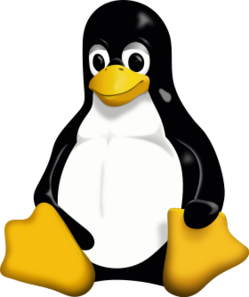
\includegraphics[width=.08\textwidth]{logo-tux.png}\hfill
  
\includegraphics[width=.3\textwidth]{logo-unab.png}\hfill
  
\includegraphics[width=.08\textwidth]{logo-python.png}
}

\makeatletter
\setbeamertemplate{title page}{
  \begin{minipage}[b][\paperheight]{\textwidth}
    \vfill%
    \ifx\inserttitle\@empty\else\usebeamertemplate*{title}\fi
    \ifx\insertsubtitle\@empty\else\usebeamertemplate*{subtitle}\fi
    \usebeamertemplate*{title separator}
    \ifx\beamer@shortauthor\@empty\else\usebeamertemplate*{author}\fi
    \ifx\insertdate\@empty\else\usebeamertemplate*{date}\fi
    \ifx\insertinstitute\@empty\else\usebeamertemplate*{institute}\fi
    \vfill
    \ifx\inserttitlegraphic\@empty\else\inserttitlegraphic\fi
    \vspace*{1cm}
  \end{minipage}
}
\makeatother


\makeatletter
\setlength{\metropolis@titleseparator@linewidth}{2pt}
\setlength{\metropolis@progressonsectionpage@linewidth}{2pt}
\setlength{\metropolis@progressinheadfoot@linewidth}{2pt}
\makeatother


\begin{document}

\myfront{}

\begin{frame}
  \titlepage
\end{frame}

\begin{frame}
  \frametitle{Resumen - Parte 2 (Semana 2)}
  \tableofcontents
\end{frame}

%----------------------------------------------------------------------------------------
%   PRESENTATION SLIDES
%----------------------------------------------------------------------------------------
\metroset{block=fill}

%------------------------------------------------
\section{El intérprete Python}

\begin{frame}{El intérprete Python}
\begin{itemize}
	\item Python es un lenguaje de programación interpretado, orientado a objeto y de alto nivel. 
	\item Es fácil de aprender y muy poderoso.
	\item Nos permite enfocarnos en “pensar como un programador” más que en detalles complejos del lenguaje.
\end{itemize}
\end{frame}

\begin{frame}[fragile]{Código "Hola Mundo" en varios lenguajes}
\begin{columns}[c]
	\column{.45\textwidth}
\begin{minted}
[
frame=lines,
framesep=2mm,
baselinestretch=1.2,
bgcolor=LightGray,
fontsize=\footnotesize
]
{C++}
// C++
#include <iostream>
int main(){
  std::cout << "Hola mundo!";
}
\end{minted}

\begin{minted}
[
frame=lines,
framesep=2mm,
baselinestretch=1.2,
bgcolor=LightGray,
fontsize=\footnotesize
]
{python}
# Python
print("Hola mundo")
\end{minted}

	\column{.52\textwidth}
\begin{minted}
[
frame=lines,
framesep=2mm,
baselinestretch=1.2,
bgcolor=LightGray,
fontsize=\footnotesize
]
{cs}
// C#
using System;
namespace HelloWorld {
  class Hello {
    static void Main() {
      Console.WriteLine("Hola Mundo!");
      Console.ReadKey();
    }
  }
}
\end{minted}

\end{columns}
\end{frame}

\begin{frame}{Ambientes de desarrollo}
\begin{itemize}
	\item Un programa en Python es una lista de instrucciones.
	\item IDEs comunes: Jupyter, VSCode, Google Colab, CoCalc, etc.
	\item En este curso usaremos principalmente terminal de Linux + editor Vim, por sus ventajas en entornos remotos.
\end{itemize}
\end{frame}

\begin{frame}[fragile]{Ejecución de programas Python}
\begin{itemize}
	\item Por convención, se nombran con la extensión \texttt{.py}.  
	\item Puedes (opcionalmente) especificar el intérprete en la primera línea:
\begin{minted}{python}
#!/usr/bin/python
x=1
print(x)
\end{minted}
	\item Ejecutar:
\begin{minted}{bash}
./programa1.py
# O bien
python programa1.py
\end{minted}
\end{itemize}
\end{frame}

%------------------------------------------------
\subsection{Variables, asignaciones y tipos}

\begin{frame}{Variables, asignaciones y tipos}
\begin{itemize}
	\item Las variables son contenedores de valores (números, texto, etc.).
	\item Se asignan con el operador “=”.
	\begin{example}
\texttt{x=1.5}
	\end{example}
	\item Tipos principales: \textbf{entero, flotante, complejo, string}.
\end{itemize}
\end{frame}

\begin{frame}{Más sobre variables}
\begin{itemize}
	\item Nombres de variables pueden contener letras, números y “\_”, pero no pueden empezar con un número.
	\item Mayúsculas y minúsculas son distintas (\texttt{X} vs \texttt{x}).
	\item Existen palabras reservadas: \texttt{if, else, while, print, class, import, …}.
\end{itemize}
\end{frame}

\begin{frame}[fragile]{Declaraciones de entrada y salida (I/O)}
\begin{itemize}
	\item \texttt{print()} para mostrar valores por pantalla.
	\begin{minted}{python}
x=1
print("El valor de x es", x)
	\end{minted}
	\item \texttt{input()} para leer valores del usuario (por defecto regresa strings).
\end{itemize}
\end{frame}

\begin{frame}[fragile]{Ejemplo simple de I/O}
\begin{minted}{python}
#!/usr/bin/python
tmp = input("Introduzca el valor de x: ")
x = float(tmp)
print("El valor de x es:", x)
\end{minted}
\end{frame}

%------------------------------------------------
\subsection{Aritmética}

\begin{frame}{Aritmética en Python}
\begin{itemize}
	\item +, -, *, /, ** (potencia).
	\item // (división entera), \% (módulo).
	\item \texttt{x += 1} equivale a \texttt{x = x + 1}.
\end{itemize}
\end{frame}

\begin{frame}[fragile]{Algunos ejemplos}
\begin{minted}{python}
x, y = 1, 2.5   # Asignación múltiple
x += 3         # x = x + 3
z = x**2 - 10  # potencia y resta
print("El valor de z es", z)
\end{minted}
\end{frame}

%------------------------------------------------
% ACTIVIDAD / EJEMPLO
%------------------------------------------------
\begin{frame}{Actividad Sugerida: Practicando Python Básico}
\begin{itemize}
    \item \textbf{Objetivo:} Familiarizarse con la sintaxis y tipos en Python.
    \item \textbf{Instrucciones:}
    \begin{enumerate}
        \item Crea un archivo \texttt{hola.py} que pida tu nombre y lo imprima con un saludo.
        \item Agrega dos variables numéricas, suma sus valores y muéstralo en pantalla.
        \item Asegúrate de especificar el intérprete en la primera línea (opcional, según tu entorno).
    \end{enumerate}
    \item \textbf{Conclusión:} Practicar la lectura de datos, la impresión y operaciones aritméticas sencillas.
\end{itemize}
\end{frame}

\begin{frame}
\Huge{\centerline{Fin de la Parte 2}}
\end{frame}

\end{document}

